\documentclass{article}
\usepackage[utf8]{inputenc}
\usepackage[spanish]{babel}

\usepackage{graphicx} % Required for inserting images
\usepackage{imakeidx}
\usepackage{amssymb, amsmath}
\usepackage{listings}
\usepackage{xcolor}
\usepackage{hyperref}
\usepackage{amssymb} % Para símbolos
\usepackage{fontawesome5} % Para emojis y otros símbolos
\makeindex
\setlength{\parindent}{12pt}

\definecolor{darkgreen}{RGB}{0, 150, 0}

% Para poner código de python en el documento
\lstdefinestyle{mystyle}{
  backgroundcolor=\color{white},
  commentstyle=\color{darkgreen},
  keywordstyle=\color{blue},
  numberstyle=\tiny\color{gray},
  stringstyle=\color{red},
  basicstyle=\ttfamily,
  breaklines=true,
  numbers=left,
  numbersep=5pt,
  showstringspaces=false,
  language=Python
}


% Márgenes de página
\usepackage[left=2.5cm, right=2.5cm, top=3cm, bottom=3cm]{geometry}

% Fuente y formato
\usepackage[T1]{fontenc} % Para las ñ y letras con tilde
\usepackage{times}
\usepackage{microtype} % Mejora el espaciado de las palabras

% Encabezado y pie de página
\usepackage{fancyhdr}
\pagestyle{fancy}
\fancyhf{} % Borra el encabezado y pie de página existentes
\rhead{Rubén Nogueras González \& Pelayo Huerta Mijares}
\rfoot{\thepage}


\begin{document}
    \begin{titlepage}
    \centering
    {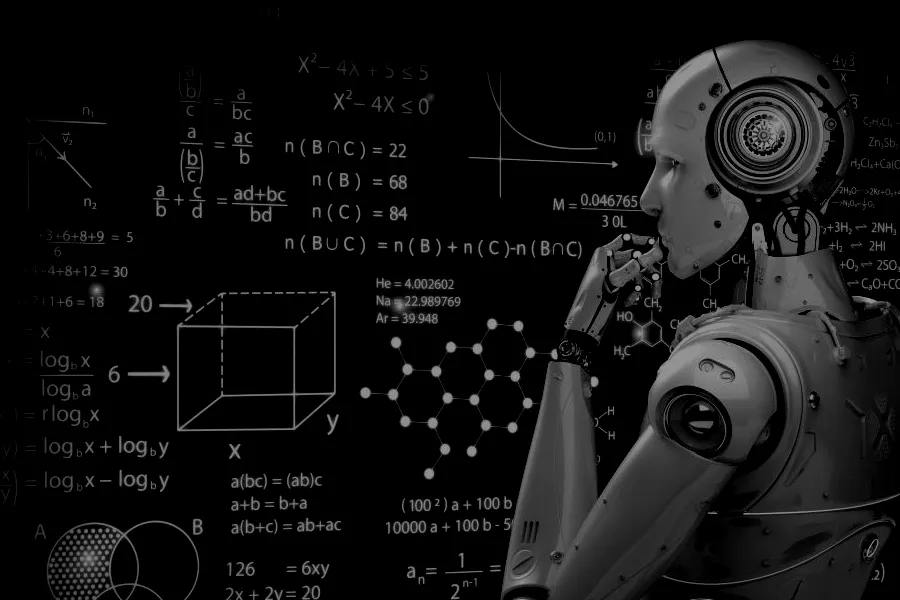
\includegraphics[width=0.5\textwidth]{portada.png}\par}
    \vspace{1cm}
    {\bfseries\LARGE Universidad Alfonso X \par}
    \vspace{3cm}
    {\scshape\Huge Técnicas de Optimización y Control \par}
    \vspace{2cm}
    {\itshape\Large Práctica 14 \par}
    \vspace{1cm}
    {\Large Autores: \par}
    {\Large Pelayo Huerta Mijares \par}
    {\Large Rubén Nogueras González \par}
    \vfill
    {\Large Diciembre 2023 \par}
    \end{titlepage}

\section{Lago Congelado (Frozen Lake)}

\vspace{1cm}


El juego Frozen Lake consiste en llevar a un agente desde un punto inicial a un objetivo en un entorno de mosaicos que representan un lago con áreas seguras y trampas. El agente puede moverse hacia la izquierda, derecha, arriba o abajo, evitando caer en los agujeros mientras busca llegar al objetivo con la menor cantidad de movimientos.

\vspace{0.5cm}

\begin{align*}
    S F F F &\: &\text{(S: punto de inicio, seguro)} \\
    F H F H  &\: &\text{F: superficie congelada, seguro)} \\
    F F F H &\: &\text{H: agujero, atrapado para siempre)} \\
    H F F G &\: &\text{G: objetivo, seguro)}
\end{align*}

\vspace{0.5cm}

Los mosaicos del juego son marcados como superficies congeladas seguras (indicadas con una marca de verificación) o agujeros peligrosos (indicados con una cruz). A pesar de que existen múltiples formas de llegar al objetivo, el desafío es hacerlo en la menor cantidad de acciones posibles. Por ejemplo, aunque se puedan encontrar diferentes rutas para llegar al objetivo, algunas pueden dar vueltas innecesarias antes de llegar al objetivo, lo cual no cumple con el requisito de minimizar los movimientos.

\vspace{0.5cm}

Para empezar, se utiliza la biblioteca 'gym' para inicializar el entorno del juego. Hay dos versiones disponibles: una con hielo resbaladizo, donde las acciones pueden ser ignoradas ocasionalmente por el agente, y otra sin esta característica. Comenzamos con la versión sin hielo resbaladizo, ya que es más sencillo de entender y abordar.

\vspace{1cm}

\section{Q-Table}

\vspace{1cm}

En el entorno Frozen Lake, hay 16 estados distintos y 4 acciones posibles para cada uno: ir izquierda, abajo, derecha y arriba. Para tomar decisiones informadas en cada estado, asignamos valores de calidad a las acciones. Esto se logra mediante una tabla Q, que enumera los estados en filas y las acciones en columnas.

\vspace{0.5cm}

Cada celda de la tabla Q contiene un valor Q(s, a), representando la calidad de la acción 'a' en el estado 's'. El valor más alto indica la mejor acción a tomar en un estado dado.

\vspace{0.5cm}

\begin{center}
\begin{tabular}{|c|c|c|c|c|}
\hline
Estado & $\leftarrow$ IZQUIERDA & $\downarrow$ ABAJO & $\rightarrow$ DERECHA & $\uparrow$ ARRIBA \\
\hline
0 & $Q(0, \leftarrow)$ & $Q(0, \downarrow)$ & $Q(0, \rightarrow)$ & $Q(0, \uparrow)$ \\
1 & $Q(1, \leftarrow)$ & $Q(1, \downarrow)$ & $Q(1, \rightarrow)$ & $Q(1, \uparrow)$ \\
2 & $Q(2, \leftarrow)$ & $Q(2, \downarrow)$ & $Q(2, \rightarrow)$ & $Q(2, \uparrow)$ \\
... & ... & ... & ... & ... \\
14 & $Q(14, \leftarrow)$ & $Q(14, \downarrow)$ & $Q(14, \rightarrow)$ & $Q(14, \uparrow)$ \\
15 & $Q(15, \leftarrow)$ & $Q(15, \downarrow)$ & $Q(15, \rightarrow)$ & $Q(15, \uparrow)$ \\
\hline
\end{tabular}
\end{center}

\vspace{0.5cm}

Esta tabla inicialmente se llena con valores de cero, ya que aún no se han calculado los valores de calidad para cada acción en cada estado. Es esencial para nuestro agente, ya que al estar en un estado particular, puede consultar esta tabla para tomar la acción con el valor de calidad más alto.

\vspace{0.5cm}

Vamos a crear nuestra tabla Q y llenarla con ceros ya que aún no tenemos idea del valor de cada acción en cada estado.

\vspace{0.5cm}

\begin{lstlisting}[style=mystyle]
    import gym
    import random
    import numpy as np
    
    # Initialize the non-slippery Frozen Lake environment
    environment = gym.make("FrozenLake-v1", is_slippery=False, render_mode="rgb_array")
    environment.reset()
    environment.render()
    
    # Initialize Q-table with zeros
    # Our table has the following dimensions:
    # (rows x columns) = (states x actions) = (16 x 4)
    qtable = np.zeros((16, 4))
    
    # Alternatively, the gym library can also directly
    # give us the number of states and actions using 
    # "env.observation_space.n" and "env.action_space.n"
    nb_states = environment.observation_space.n  # = 16
    nb_actions = environment.action_space.n      # = 4
    qtable = np.zeros((nb_states, nb_actions))
    
    # Let's see how it looks
    print('Q-table =')
    print(qtable)
\end{lstlisting}

\vspace{0.5cm}

\begin{center}
    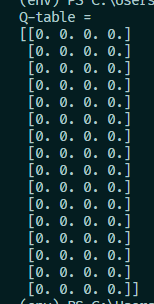
\includegraphics[width=0.5\linewidth]{QTable_ceros.png}
\end{center}

\vspace{0.5cm}

En este momento, el agente se encuentra en el estado inicial $S$. En esta posición, solo tiene dos opciones de movimiento disponibles: ir hacia la derecha ($\rightarrow$ DERECHA) o hacia abajo ($\downarrow$ ABAJO). Aunque el agente técnicamente puede realizar las acciones de moverse hacia arriba ($\uparrow$ ARRIBA) o hacia la izquierda ($\leftarrow$ IZQUIERDA), estas acciones no resultarán en un cambio de estado. En otras palabras, no hay restricciones impuestas sobre qué acciones puede realizar el agente; sin embargo, naturalmente comprenderá que algunas de estas acciones no tienen efecto en su posición actual y no cambiarán su estado.

\vspace{0.5cm}

La biblioteca gym implementa un metodo para elegir de manera random una acción, por lo que nos ahorramos el tener que usar la librería random, haciendo uso del siguiente comando:

\vspace{0.5cm}

\begin{lstlisting}[style=mystyle]
    environment.action_space.sample()

\end{lstlisting}

\vspace{0.5cm}

\begin{center}
    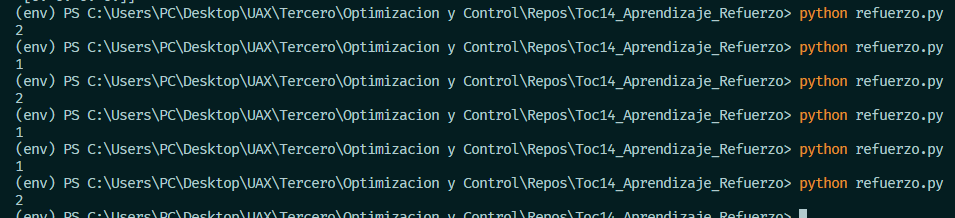
\includegraphics[width=0.75\linewidth]{image.png}
    
\end{center}

\vspace{0.5cm}

Vemos que la salida varía entre 1 y 2, ¿Por qué puede ser esto? y, ¿Por qué es un número?

\vspace{0.5cm}

\begin{center}
$\leftarrow$ LEFT = 0 \\
$\downarrow$ DOWN = 1 \\
$\rightarrow$ RIGHT = 2 \\
$\uparrow$ UP = 3
\end{center}

\vspace{0.5cm}

De esta manera, la biblioteca gym conecta números con las direcciones del agente en el juego. Vamos a intentar mover el agente para que haga un movimiento hacia la derecha:

\vspace{0.5cm}

\begin{lstlisting}[style=mystyle]
    environment.step(2)environment.render()

\end{lstlisting}

\vspace{0.5cm}

Y el resultado es:

\vspace{0.5cm}

\begin{center}
    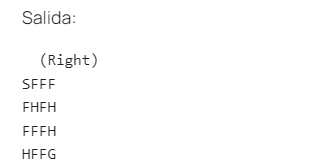
\includegraphics[width=0.75\linewidth]{mov_der.png}
\end{center}

\vspace{0.5cm}

Ahora que comprendemos la interacción con nuestro entorno en Gym, regresemos al algoritmo. En el aprendizaje por refuerzo, los agentes reciben recompensas del entorno cuando logran cumplir un objetivo específico. En el contexto de Frozen Lake, el agente solo recibe una recompensa cuando alcanza el estado G (consultar el código fuente). Esta recompensa está predefinida en el entorno y está fuera de nuestro control: proporciona un valor de 1 cuando el agente llega al estado G y un valor de 0 en caso contrario.

\vspace{0.5cm}

Cada vez que implementemos una acción, imprimiremos esta recompensa. El método step(action) proporciona esta recompensa.

\vspace{0.5cm}

\begin{lstlisting}[style=mystyle]
    # 1. Randomly choose an action using action_space.sample()
    action = environment.action_space.sample()
    
    # 2. Implement this action and move the agent in the desired direction
    new_state, reward, done, info = environment.step(action)
    
    # Display the results (reward and map)
    environment.render()
    print(f'Reward = {reward}')
\end{lstlisting}

\vspace{0.5cm}

\begin{center}
    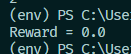
\includegraphics[width=0.5\linewidth]{reward0.png}
\end{center}

\vspace{0.5cm}

La situación es desafiante: la recompensa actual es 0, y solo un estado específico ofrece una recompensa positiva en todo el juego. ¿Cómo podemos encontrar la ruta correcta si solo sabemos al final si hemos tenido éxito? Para obtener una recompensa, debemos confiar en la casualidad de encontrar la secuencia correcta de acciones. Lamentablemente, esa es la naturaleza del proceso: la tabla Q se llena de ceros hasta que el agente encuentre la meta G por casualidad.

\vspace{0.5cm}

Sería más fácil si hubiera recompensas más pequeñas durante el camino hacia la meta G. Sin embargo, este es un desafío clave del aprendizaje por refuerzo: las recompensas son escasas, lo que dificulta entrenar a los agentes cuando la única recompensa está al final de una larga secuencia de acciones. Se han propuesto técnicas para abordar esto, pero exploraremos estas soluciones en otro momento.

\vspace{1cm}

\section{Q-Aprendizaje}

\vspace{1cm}

Volvamos al problema. En este juego, encontrar la meta G es una cuestión de suerte. Pero una vez que la alcanzamos, ¿cómo retrocedemos esa información al estado inicial? El algoritmo Q-learning ofrece una solución inteligente a este dilema. Actualiza los valores de nuestros pares estado-acción (representados en la tabla Q) considerando la recompensa por alcanzar el próximo estado y el máximo valor en ese estado.

\vspace{0.5cm}

Supongamos que obtenemos una recompensa de 1 al llegar a G. El valor del estado junto a G (denominémoslo G-1) se incrementa gracias a esta recompensa. Ahora, cada vez que el agente esté en un estado cercano a G-1, aumentará el valor de G-1, y así sucesivamente hasta alcanzar el estado inicial S.

\vspace{0.5cm}

Intentemos encontrar la fórmula de actualización para propagar los valores desde G hasta S. Los valores representan la calidad de una acción en un estado específico (0 si es pobre, 1 si es la mejor posible). Queremos actualizar el valor de la acción en el estado (por ejemplo, cuando el agente está en el estado inicial S). Esta actualización se realiza con la fórmula:

\vspace{0.5cm}

\[
Q_{nuevo}(s, a) = Q_{viejo}(s, a) + \alpha \cdot \left( R + \gamma \cdot \max_{a'} Q_{viejo}(s', a') - Q_{viejo}(s, a) \right)
\]

\vspace{0.5cm}

Donde:
\(Q_{nuevo}\) es el nuevo valor,
\(Q_{viejo}\) es el valor existente,
\(\alpha\) es la tasa de aprendizaje (entre 0 y 1),
\(R\) es la recompensa para el siguiente estado,
\(\gamma\) es el factor de descuento (entre 0 y 1).

\vspace{0.5cm}

Con el algoritmo Q-learning, la actualización se realiza así:

\vspace{0.5cm}

\[
Q_{nuevo}(s, a) = Q_{viejo}(s, a) + \alpha \cdot \left( R + \gamma \cdot \max_{a'} Q_{viejo}(s', a') - Q_{viejo}(s, a) \right)
\]

\vspace{0.5cm}

Es crucial encontrar un equilibrio entre el conocimiento pasado (\(\alpha\)) y el peso de las recompensas futuras (\(\gamma\)). Luego, entrenar al agente implica:

\vspace{0.5cm}

1. Elegir una acción aleatoria si los valores en el estado actual son ceros, o tomar la acción con el mayor valor.
2. Implementar la acción y actualizar el valor del estado actual según la fórmula de Q-learning.
3. Repetir hasta que el agente alcance la meta o se atasque.

\vspace{0.5cm}

Este proceso se repite durante varios episodios, reiniciando el entorno después de cada uno. Graficar los resultados puede ayudar a visualizar el progreso del agente.

\vspace{0.5cm}

\begin{lstlisting}[style=mystyle]
    plt.rcParams['figure.dpi'] = 300
    plt.rcParams.update({'font.size': 17})
    
    # We re-initialize the Q-table
    qtable = np.zeros((environment.observation_space.n, environment.action_space.n))
    
    # Hyperparameters
    episodes = 1000        # Total number of episodes
    alpha = 0.5            # Learning rate
    gamma = 0.9            # Discount factor
    
    # List of outcomes to plot
    outcomes = []
    
    print('Q-table before training:')
    print(qtable)
    
    # Training
    for _ in range(episodes):
        state = environment.reset()
        state = int(state[0])
        done = False
    
        # By default, we consider our outcome to be a failure
        outcomes.append("Failure")
    
        # Until the agent gets stuck in a hole or reaches the goal, keep training it
        while not done:
            # Choose the action with the highest value in the current state
            if np.max(qtable[state]) > 0:
              action = np.argmax(qtable[state])
    
            # If there's no best action (only zeros), take a random one
            else:
              action = environment.action_space.sample()        
        
            # Implement this action and move the agent in the desired direction
            new_state, reward, done, truncated, info = environment.step(action)
    
    
            # Update Q(s,a)
            qtable[state, action] = qtable[state, action] + \
                                    alpha * (reward + gamma * np.max(qtable[new_state]) - 
                                    qtable[state, action])
                 
            # Update our current state
            state = new_state
    
            # If we have a reward, it means that our outcome is a success
            if reward:
              outcomes[-1] = "Success"
    
    print()
    print('===========================================')
    print('Q-table after training:')
    print(qtable)
    
    # Plot outcomes
    plt.figure(figsize=(12, 5))
    plt.xlabel("Run number")
    plt.ylabel("Outcome")
    ax = plt.gca()
    plt.bar(range(len(outcomes)), outcomes, width=1.0)
    plt.show()    
\end{lstlisting}

\vspace{0.5cm}

\begin{center}
    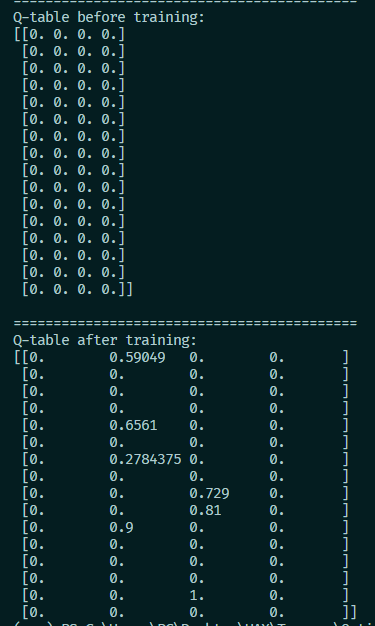
\includegraphics[width=0.5\linewidth]{aftertraining.png}
\end{center}

\vspace{0.5cm}

\begin{center}
    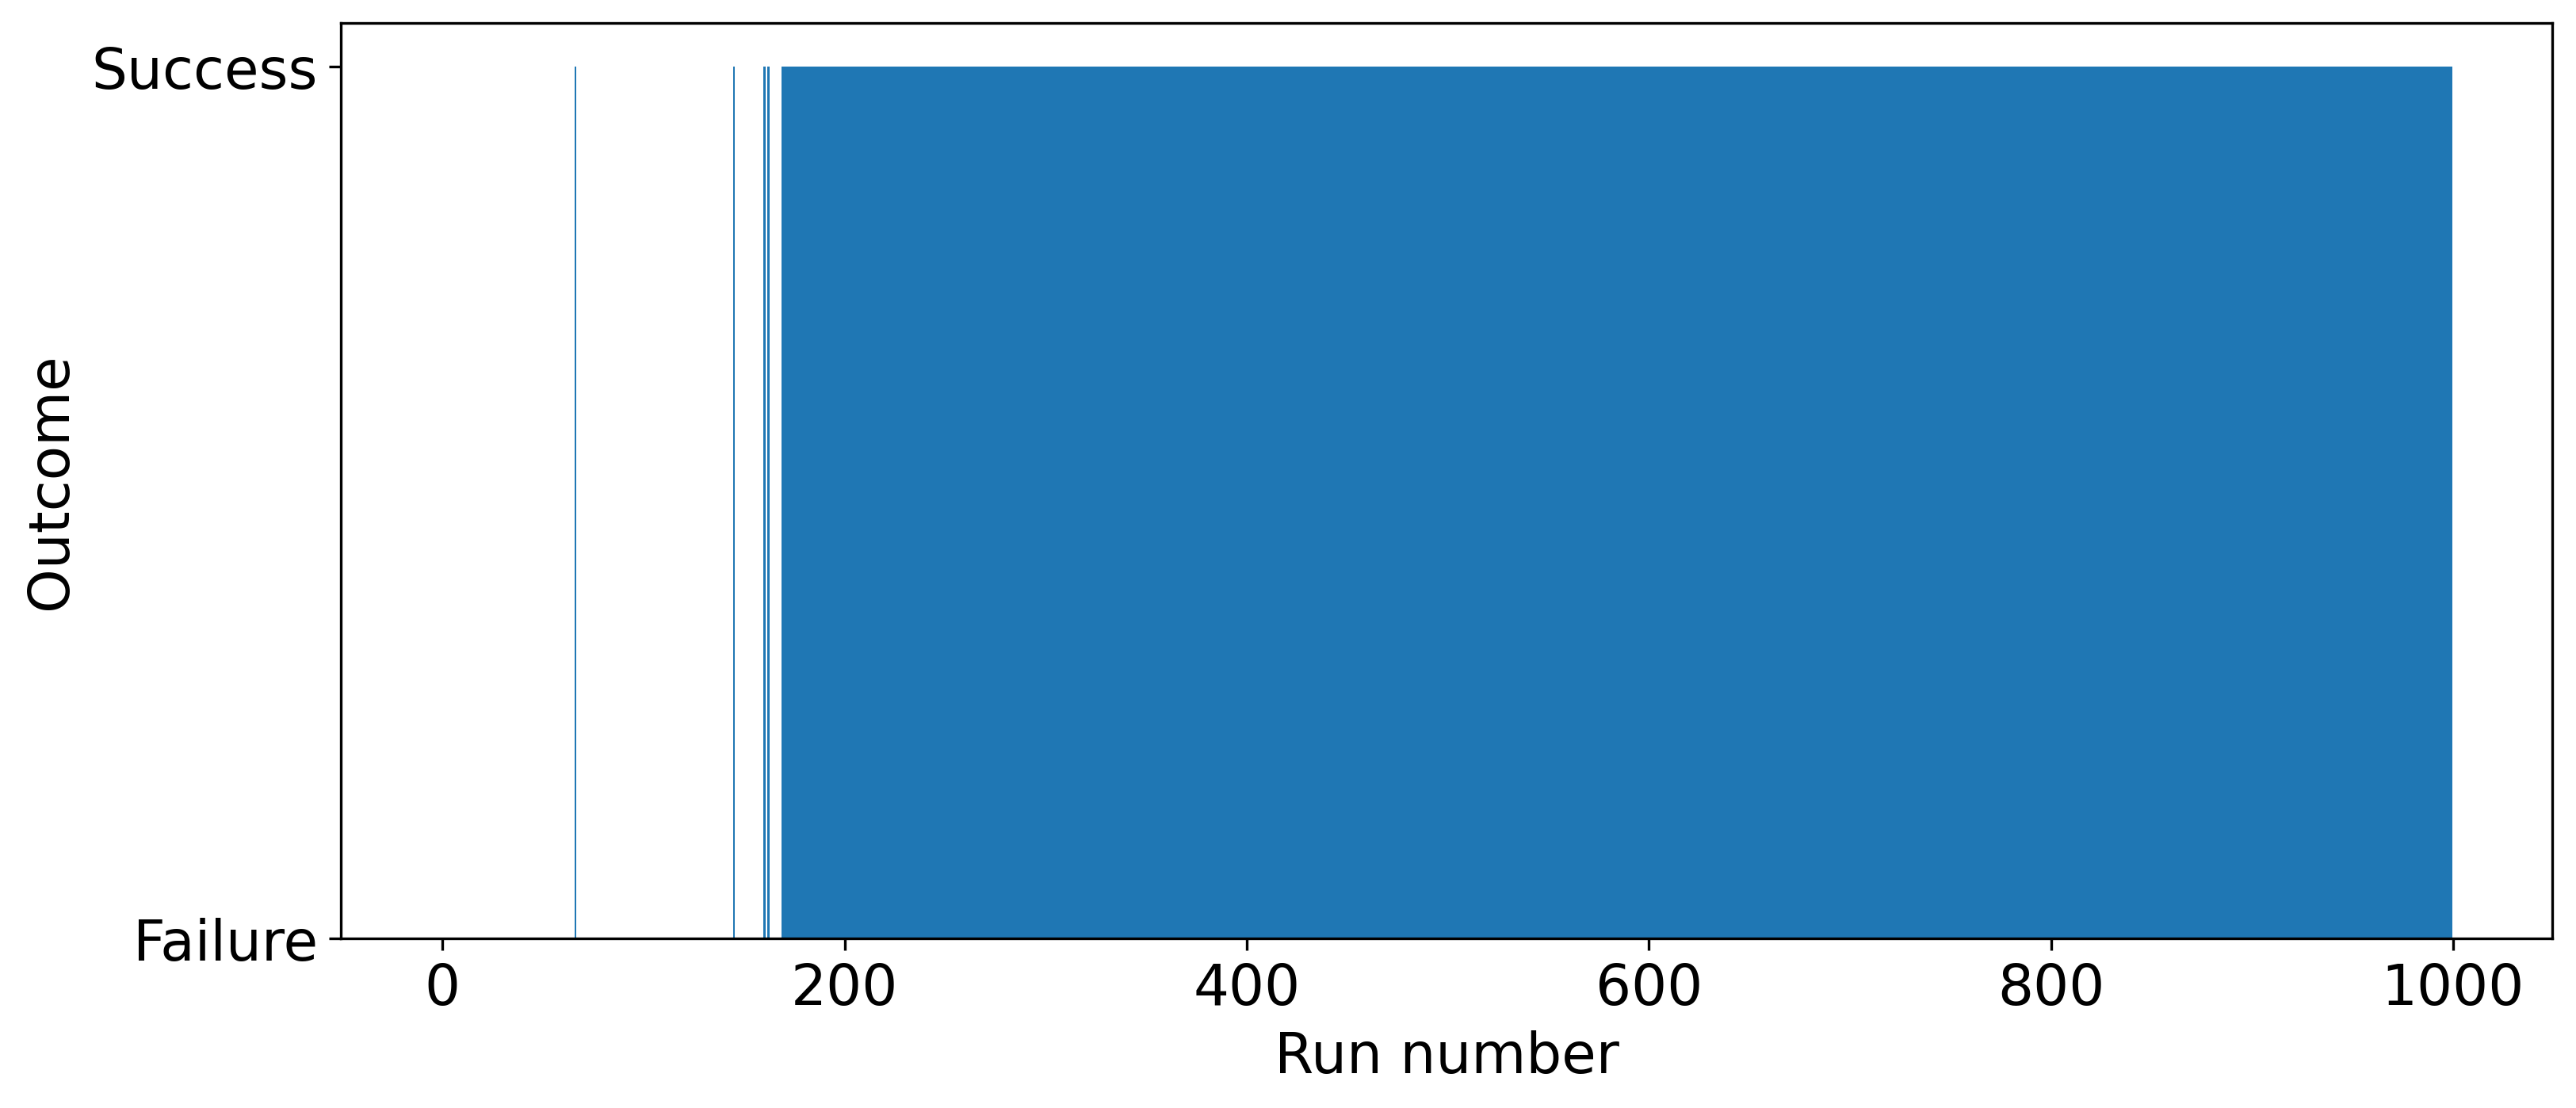
\includegraphics[width=0.8\linewidth]{Figure_1.png}
\end{center}

\vspace{0.5cm}

Después de entrenar al agente, observamos un progreso significativo. Al principio, le costó encontrar la meta, pero con el tiempo, logró alcanzarla de manera más consistente. La tabla Q resultante muestra las acciones aprendidas por el agente para lograr su objetivo. Evaluamos su rendimiento en 100 episodios para medir su tasa de éxito en llegar a la meta.

\vspace{0.5cm}

\begin{lstlisting}[style=mystyle]
    episodes = 100
    nb_success = 0
    
    # Evaluation
    for _ in range(episodes):
        state = environment.reset()
        state = int(state[0])
        done = False
        
        # Until the agent gets stuck or reaches the goal, keep training it
        while not done:
            # Choose the action with the highest value in the current state
            if np.max(qtable[state]) > 0:
              action = np.argmax(qtable[state])
    
            # If there's no best action (only zeros), take a random one
            else:
              action = environment.action_space.sample()
              
            # Implement this action and move the agent in the desired direction
            new_state, reward, done, truncated, info = environment.step(action)
           
            # Update our current state
            state = new_state
    
            # When we get a reward, it means we solved the game
            nb_success += reward
    
    # Let's check our success rate!
    print (f"Success rate = {nb_success/episodes*100}%")
\end{lstlisting}

\vspace{0.5cm}

\begin{center}
    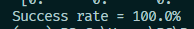
\includegraphics[width=0.75\linewidth]{successrate.png}
\end{center}

\vspace{0.5cm}

Vemos que hemos conseguido una tasa de exito del 100\%. Con esto queda resuelto el Frozen Lake no resbaladizo.

\vspace{0.5cm}

Además podemos ver los movimientos del agente y mostrar la secuencia de acciones para saber si se eligió la mejor:

\vspace{0.5cm}

\begin{lstlisting}[style=mystyle]
    state = environment.reset()
    state = int(state[0])
    done = False
    sequence = []
    
    while not done:
        # Choose the action with the highest value in the current state
        if np.max(qtable[state]) > 0:
          action = np.argmax(qtable[state])
    
        # If there's no best action (only zeros), take a random one
        else:
          action = environment.action_space.sample()
          
        # Add the action to the sequence
        sequence.append(action)
    
        # Implement this action and move the agent in the desired direction
        new_state, reward, done, truncated, info = environment.step(action)
    
        # Update our current state
        state = new_state
    
        # Update the render
        clear_output(wait=True)
        environment.render()
        time.sleep(1)
    
    print(f"Sequence = {sequence}")
\end{lstlisting}

\vspace{0.5cm}

\begin{center}
    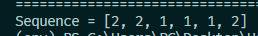
\includegraphics[width=0.75\linewidth]{optimo.png}
\end{center}

\vspace{0.5cm}

El agente ha adquirido conocimiento sobre varias secuencias correctas de acciones, por ejemplo, [2, 2, 1, 1, 1, 2], [1, 1, 2, 2, 1, 2], entre otras. Esto es particularmente interesante ya que solo hay seis acciones en estas secuencias, el mínimo número posible que identificamos. Esta situación sugiere que nuestro agente ha aprendido a resolver el juego de manera óptima.

\vspace{0.5cm}

Tomando como ejemplo la secuencia [2, 2, 1, 1, 1, 2], que corresponde a la secuencia DERECHA, DERECHA, ABAJO, ABAJO, ABAJO, DERECHA, es precisamente la secuencia que anticipamos al inicio.

\vspace{1cm}

\section{Algoritmo Epsilon-Greedy}

\vspace{1cm}

A pesar del éxito obtenido, hay un inconveniente en nuestro enfoque previo: el agente siempre elige la acción con el valor más alto. Esto significa que las otras acciones nunca se exploran ni actualizan en su valor, lo cual podría limitar el aprendizaje del agente. ¿Qué pasaría si alguna de estas acciones no exploradas fuera mejor que la opción que el agente siempre elige? ¿No deberíamos incentivar al agente para que explore nuevas acciones y así mejorar?

\vspace{0.5cm}

En resumen, deseamos que nuestro agente:

\begin{itemize}
    \item Elija la acción más valiosa (explotación).
    \item Seleccione ocasionalmente acciones aleatorias para descubrir alternativas potencialmente mejores (exploración).
\end{itemize}

\vspace{0.5cm}

Queremos equilibrar estos comportamientos: si el agente solo explota, no aprenderá más, pero si solo explora, el entrenamiento será ineficiente. Por ello, ajustaremos un parámetro con el tiempo: al principio, se preferirá la exploración extensa, pero a medida que el agente conozca mejor el entorno, la exploración se reducirá. Este parámetro, denominado épsilon, controla el nivel de aleatoriedad en la selección de acciones.

\vspace{0.5cm}

Este enfoque se conoce como algoritmo epsilon-greedy, donde epsilon es el parámetro clave. Es un método sencillo pero muy efectivo para lograr un equilibrio adecuado. En cada decisión, el agente tiene una probabilidad $\epsilon$ de seleccionar aleatoriamente una acción y una probabilidad de 1 menos $\epsilon$ de elegir la acción más valiosa. Podemos reducir gradualmente el valor de $\epsilon$ al final de cada episodio, ya sea en cantidades fijas (decaimiento lineal) o en función de su valor actual (decaimiento exponencial).

\vspace{0.5cm}

Vamos a ver como hacerlo en código:

\vspace{0.5cm}

\begin{lstlisting}[style=mystyle]
    # We re-initialize the Q-table
    qtable = np.zeros((environment.observation_space.n, environment.action_space.n))
    
    # Hyperparameters
    episodes = 1000        # Total number of episode
    salpha = 0.5            # Learning rate
    gamma = 0.9            # Discount factor
    epsilon = 1.0          # Amount of randomness in the action selection
    epsilon_decay = 0.001  # Fixed amount to decrease
    
    # List of outcomes to plot
    outcomes = []
    
    print('Q-table before training:')
    print(qtable)
    
    # Training
    for _ in range(episodes):
        state = environment.reset()
        state = int(state[0])
        done = False
    
        # By default, we consider our outcome to be a failure
        outcomes.append("Failure")
        
        # Until the agent gets stuck in a hole or reaches the goal, keep training it
        while not done:
            # Generate a random number between 0 and 1
            rnd = np.random.random()
            # If random number < epsilon, take a random action
            if rnd < epsilon:
              action = environment.action_space.sample()
            # Else, take the action with the highest value in the current state
            else:
              action = np.argmax(qtable[state])
            
            # Implement this action and move the agent in the desired direction
            new_state, reward, done, truncated, info = environment.step(action)
    
            # Update Q(s,a)
            qtable[state, action] = qtable[state, action] + \
                                    alpha * (reward + gamma * np.max(qtable[new_state]) - qtable[state, action])
            
            # Update our current state
            state = new_state
    
            # If we have a reward, it means that our outcome is a success
            if reward:
              outcomes[-1] = "Success"
    
        # Update epsilon
        epsilon = max(epsilon - epsilon_decay, 0)
    
    print()
    print('===========================================')
    print('Q-table after training:')
    print(qtable)
    
    # Plot outcomes
    plt.figure(figsize=(12, 5))
    plt.xlabel("Run number")
    plt.ylabel("Outcome")
    ax = plt.gca()
    plt.bar(range(len(outcomes)), outcomes, width=1.0)
    plt.show()
\end{lstlisting}

\vspace{0.5cm}

\begin{center}
    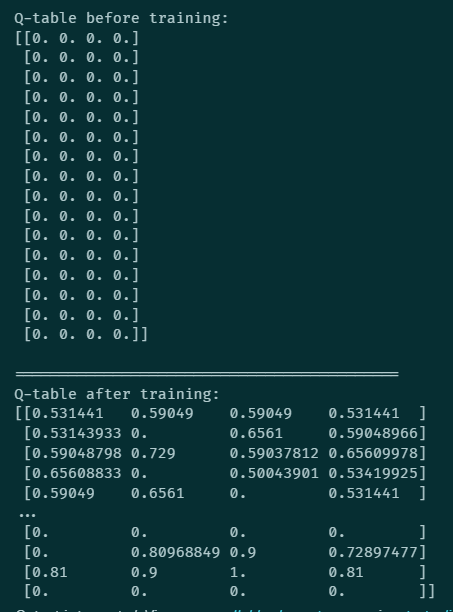
\includegraphics[width=0.5\linewidth]{trifasico.png}
\end{center}

\vspace{0.5cm}

\begin{center}
    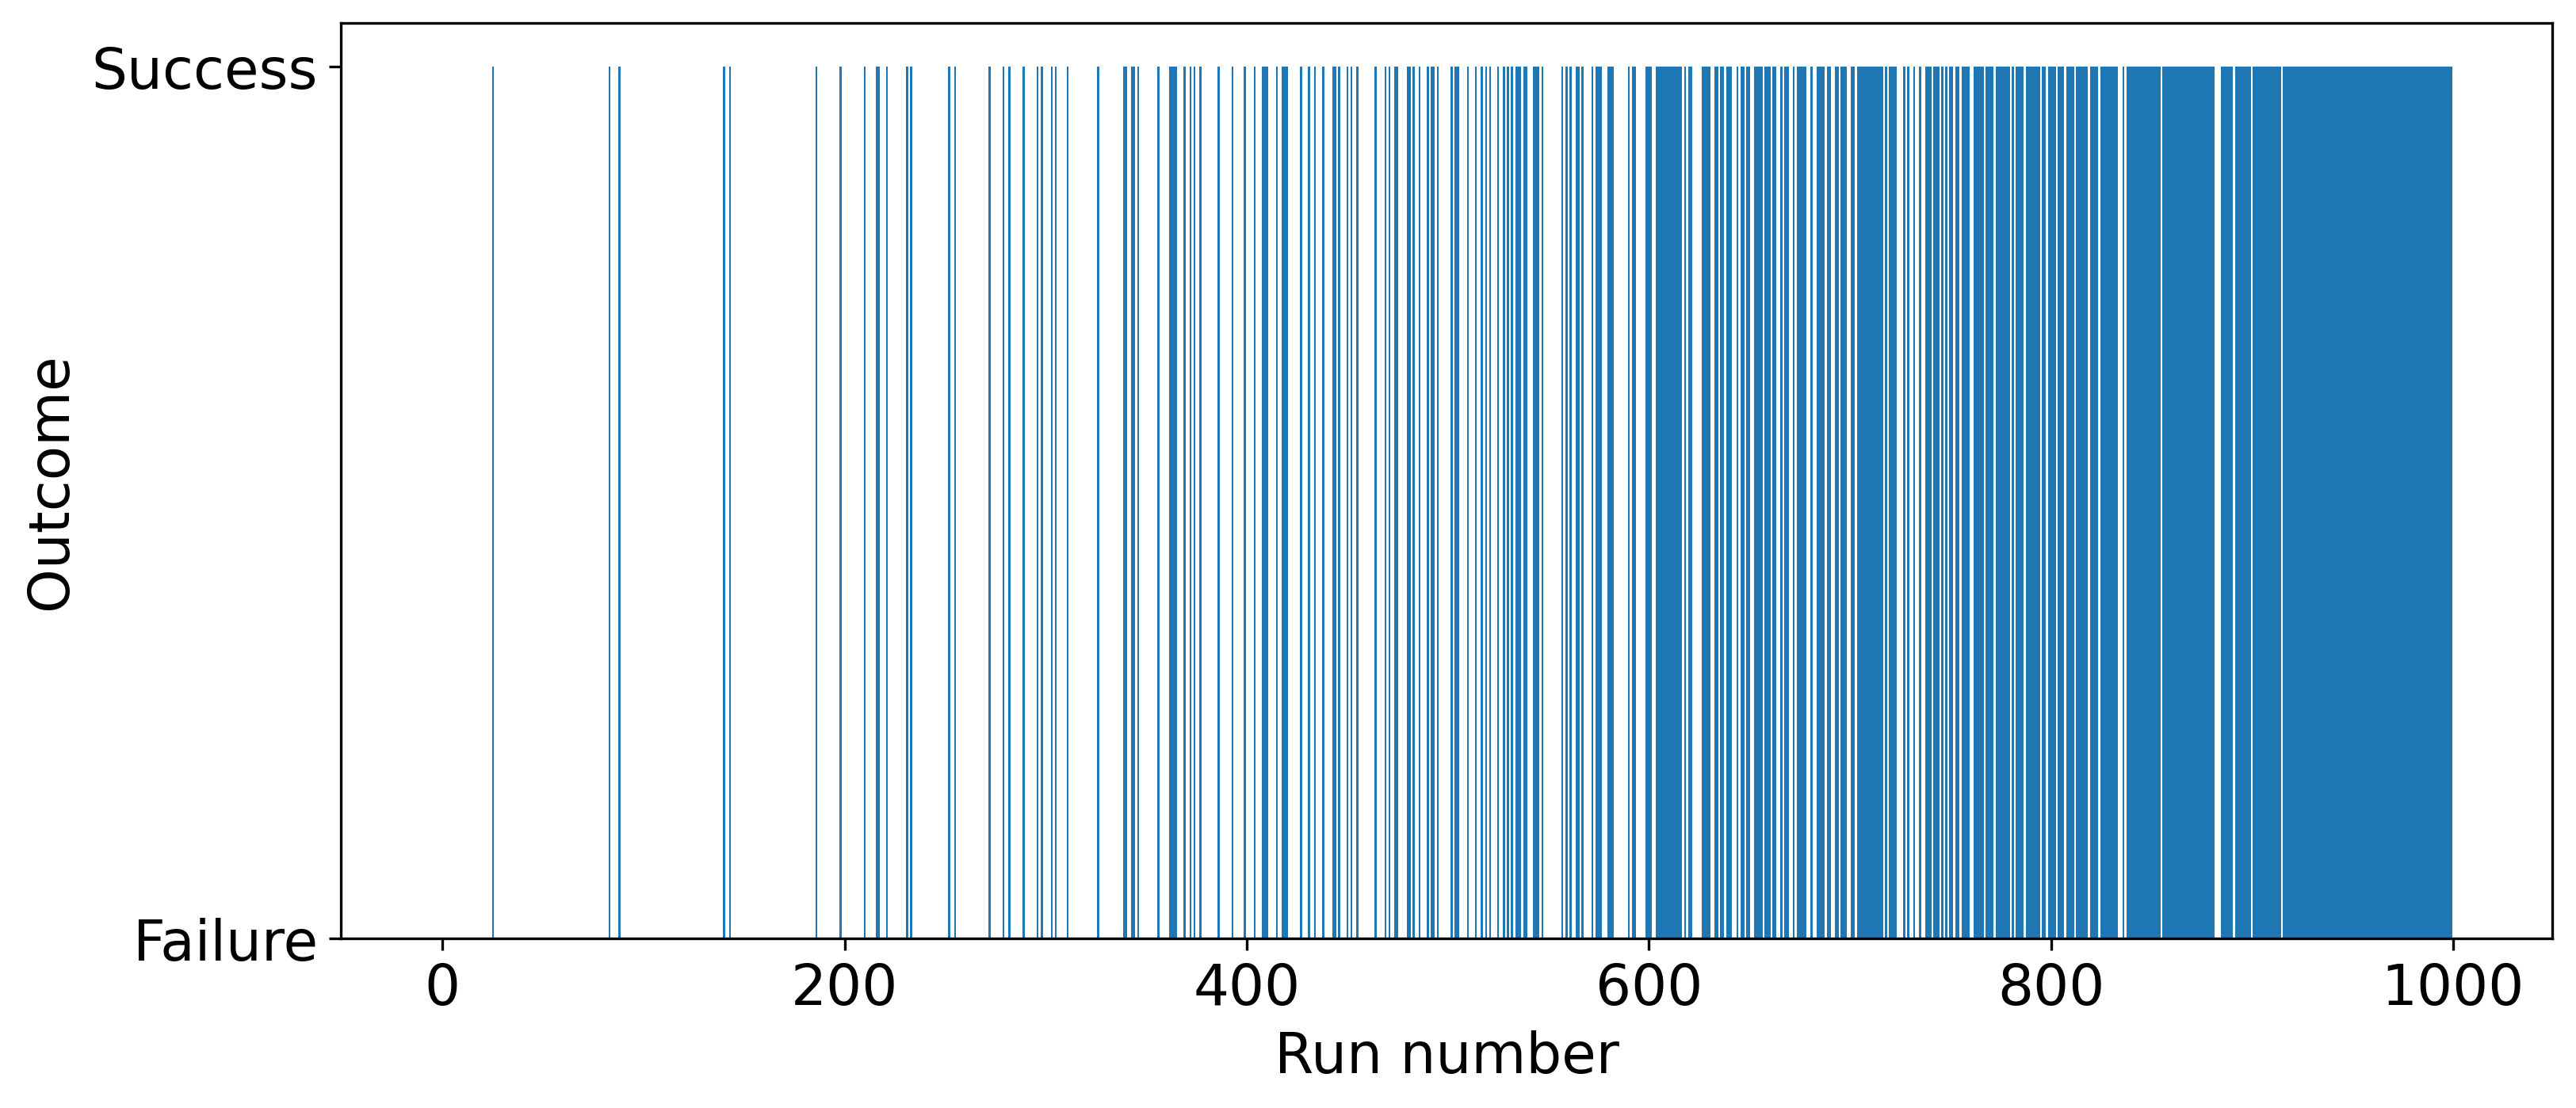
\includegraphics[width=0.75\linewidth]{jurasico.png}
\end{center}

\vspace{0.5cm}

Con estos resultados, vemos que ahora el agente ahora tarda más en ganar de manera constante, lo que indica que ha aprendido múltiples formas de alcanzar el objetivo. La tabla Q tiene más valores diferentes de cero debido a la exploración forzada de nuevos pares estado-acción. Sin embargo, para evaluar su rendimiento, deseamos ver si este agente tiene éxito como el anterior. Durante la evaluación, ya no requerimos exploración, ya que el agente está completamente entrenado. Vamos a implementarlo en código:

\vspace{0.5cm}

\begin{lstlisting}[style=mystyle]
    episodes = 100
    nb_success = 0
    
    # Evaluation
    for _ in range(100):
        state = environment.reset()
        state = int(state[0])
        done = False
       
        # Until the agent gets stuck or reaches the goal, keep training it
        while not done:
            # Choose the action with the highest value in the current state
            action = np.argmax(qtable[state])
    
            # Implement this action and move the agent in the desired direction
            new_state, reward, done, truncated, info = environment.step(action)
        
    
            # Update our current state
            state = new_state
    
            # When we get a reward, it means we solved the game
            nb_success += reward
    
    # Let's check our success rate!
    print (f"Success rate = {nb_success/episodes*100}%")
\end{lstlisting}

\vspace{0.5cm}

\begin{center}
    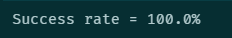
\includegraphics[width=0.75\linewidth]{no_exploracion.png}
\end{center}

\vspace{0.5cm}

Vemos que el rendimiento sigue siendo del 100 por ciento, y el modelo es ahora más flexible, ya que el agente ha aprendido varios caminos para llegar a G. Sin embargo, esto puede causar problemas en términos de rendimiento, pero es importante disponer de varias soluciones en lugar de una sola.

\vspace{1cm}

\section{Desafío: Lago helado resbaladizo}

\vspace{1cm}

Vamos a ver ahora la variante resbaladiza. Para ello, en el código, ponemos $is_slippery = True$, y el agente ahora sólo tendrá un 33\% de probabilidades de realizar el movimiento. Si fallamos, vamos aleatoriamente a una de las otras 3 acciones. Vamos a verlo en nuestro código:

\vspace{0.5cm}

\begin{lstlisting}[style=mystyle]
    # Initialize the slippery Frozen Lake
    environment = gym.make("FrozenLake-v1", is_slippery=True, render_mode="rgb_array")
    environment.reset()
    
    # We re-initialize the Q-table
    qtable = np.zeros((environment.observation_space.n, environment.action_space.n))
    
    # Hyperparameters
    episodes = 1000        # Total number of episodes
    alpha = 0.5            # Learning rate
    gamma = 0.9            # Discount factor
    epsilon = 1.0          # Amount of randomness in the action selection
    epsilon_decay = 0.001  # Fixed amount to decrease
    
    # List of outcomes to plot
    outcomes = []
    
    print('Q-table before training:')
    print(qtable)
    
    # Training
    for _ in range(episodes):
        state = environment.reset()
        state = int(state[0])
        done = False
    
        # By default, we consider our outcome to be a failure
        outcomes.append("Failure")
        
        # Until the agent gets stuck in a hole or reaches the goal, keep training it
        while not done:
            # Generate a random number between 0 and 1
            rnd = np.random.random()
    
            # If random number < epsilon, take a random action
            if rnd < epsilon:
              action = environment.action_space.sample()
    
            # Else, take the action with the highest value in the current state
            else:
              action = np.argmax(qtable[state])
           
            # Implement this action and move the agent in the desired direction
            new_state, reward, done, truncated, info = environment.step(action)
    
            # Update Q(s,a)
            qtable[state, action] = qtable[state, action] + \
                                    alpha * (reward + gamma * np.max(qtable[new_state]) - qtable[state, action])
    
           
             # Update our current state
            state = new_state
    
            # If we have a reward, it means that our outcome is a success
            if reward:
              outcomes[-1] = "Success"
    
        # Update epsilon
        epsilon = max(epsilon - epsilon_decay, 0)
    
    print()
    print('===========================================')
    print('Q-table after training:')
    print(qtable)
    
    # Plot outcomes
    plt.figure(figsize=(12, 5))
    plt.xlabel("Run number")
    plt.ylabel("Outcome")
    ax = plt.gca()
    plt.bar(range(len(outcomes)), outcomes, width=1.0)
    plt.show()
\end{lstlisting}

\vspace{0.5cm}

\begin{center}
    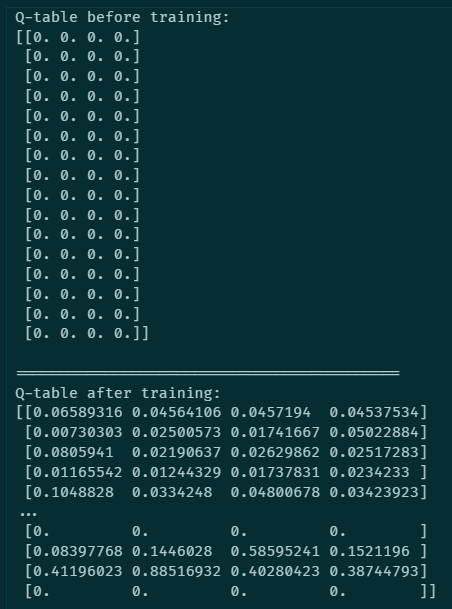
\includegraphics[width=0.5\linewidth]{resbaladizo.png}
\end{center}

\vspace{0.5cm}

\begin{center}
    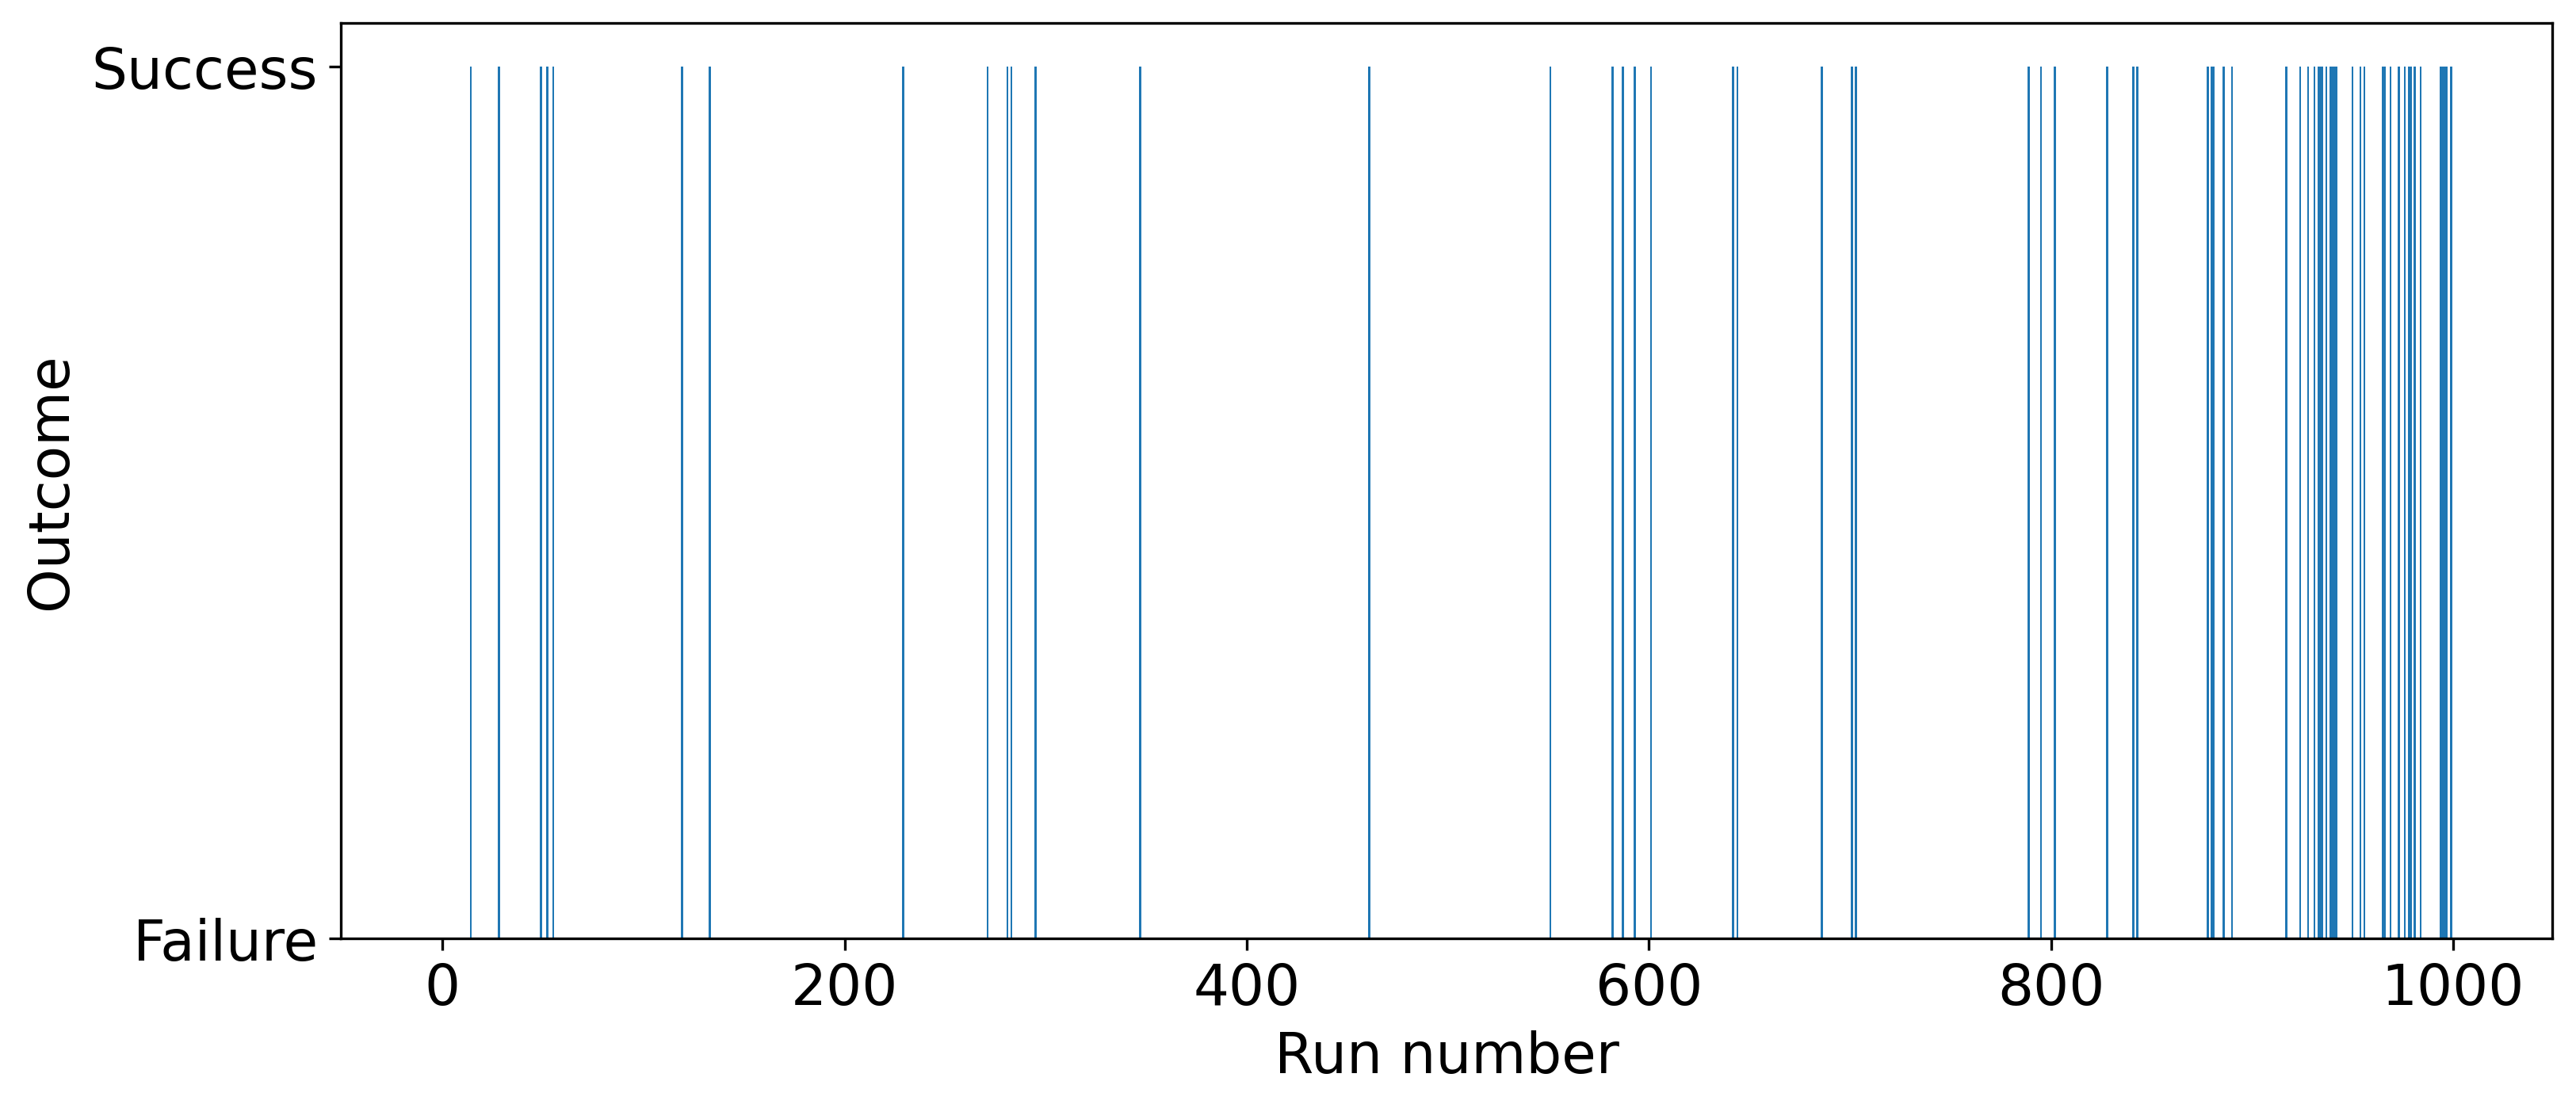
\includegraphics[width=0.75\linewidth]{resbaladizo_grafico.png}
\end{center}

\vspace{0.5cm}

Vamos a ver que ha ocurrido con la tasa de exito...

\vspace{0.5cm}

\begin{lstlisting}[style=mystyle]
    episodes = 100
    nb_success = 0
    
    # Evaluation
    for _ in range(100):
        state = environment.reset()
        state = int(state[0])
        done = False
        
        # Until the agent gets stuck or reaches the goal, keep training it
        while not done:
            # Choose the action with the highest value in the current state
            action = np.argmax(qtable[state])
    
            # Implement this action and move the agent in the desired direction
            new_state, reward, done, truncated, info = environment.step(action)
    
            # Update our current state
            state = new_state
    
            # When we get a reward, it means we solved the game
            nb_success += reward
    
    # Let's check our success rate!
    print (f"Success rate = {nb_success/episodes*100}%")
\end{lstlisting}

\vspace{0.5cm}

\begin{center}
    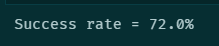
\includegraphics[width=0.75\linewidth]{resbaladizo_rate.png}
\end{center}

\vspace{0.5cm}

Podemos ver que la tasa ha empeorado, siendo ahora del 72\%. Sin embargo este porcentaje se puede aumentar ajustando unos diversos parámetros.

\vspace{1cm}

\section{Conclusión}

\vspace{1cm}

El algoritmo Q-learning es fundamental en el aprendizaje por refuerzo, un método poderoso y simple. En esta práctica:

\vspace{0.5cm}

\begin{itemize}
    \item Aprendimos a interactuar con el entorno Gym para tomar decisiones y mover a nuestro agente.
    \item Presentamos la tabla Q, que representa valores de acciones en estados específicos.
    \item Experimentamos con la fórmula de actualización del Q-learning para abordar la escasez de recompensas.
    \item Desarrollamos un proceso de entrenamiento y evaluación que resolvió el desafío Frozen Lake con una tasa de éxito del 100%.
    \item Implementamos el conocido algoritmo épsilon-greedy para equilibrar la exploración y explotación de pares de estado-acción.
\end{itemize}

\vspace{0.5cm}

Si bien el entorno Frozen Lake es simple, en entornos más complejos, el almacenamiento de la tabla Q puede ser imposible debido al gran número de estados y acciones, especialmente en entornos continuos (como Super Mario Bros. o Minecraft). Para abordar esto, una técnica popular involucra el uso de redes neuronales profundas para aproximar la tabla Q. Sin embargo, esto añade complejidad debido a la inestabilidad de las redes neuronales.

\end{document}
